\documentclass[conference]{IEEEtran}
\IEEEoverridecommandlockouts
\usepackage{cite}
\usepackage{amsmath,amssymb,amsfonts,amsthm}
\newtheorem{definition}{Definition}
\usepackage{graphicx}
\usepackage{textcomp}
\usepackage{xcolor}
\usepackage{booktabs}
\usepackage{listings}
\usepackage{url}
\usepackage{tikz}
\usetikzlibrary{arrows.meta,positioning,fit,backgrounds,shapes.geometric,topaths,calc}
\def\BibTeX{{\rm B\kern-.05em{\sc i\kern-.025em b}\kern-.08em
    T\kern-.1667em\lower.7ex\hbox{E}\kern-.125emX}}

% DSL listing style
\lstdefinestyle{causaldsl}{
  basicstyle=\ttfamily\small,
  keywordstyle=\bfseries,
  columns=fullflexible,
  breaklines=true,
  keywords={DEFINE,MODEL,CAUSAL,DAG,VARIABLE,IDENTIFY,EFFECT,OF,ON,RETURN,
            ADJUSTMENT,SETS,ANCESTORS,DESCENDANTS,MEDIATORS,COLLIDERS,
            CONFOUNDERS,BACKDOOR,PATHS,BETWEEN,AND,ESTIMATE,INTERVENE,
            COMPARE,TO,COUNTERFACTUAL,GIVEN,WHAT,WOULD,HAVE,BEEN,IF,USE,RESET,
            EXPLAIN,MINIMAL,SHOW,MODELS,WEIGHT,MEAN,NOISE}
}

% editorial notes: remove before submission
\newcommand{\TODO}[1]{\textcolor{red}{[\textbf{TODO:} #1]}}
\newcommand{\NOTE}[1]{\textcolor{blue}{[#1]}}

% notation
\newcommand{\an}{\mathrm{an}}
\newcommand{\de}{\mathrm{de}}
\newcommand{\pa}{\mathrm{pa}}
\newcommand{\ch}{\mathrm{ch}}
\newcommand{\cn}{\mathrm{cn}}
\newcommand{\forb}{\mathrm{forb}}
\newcommand{\adj}{\mathrm{adj}}
\newcommand{\dsep}{\perp\!\!\!\perp}

\begin{document}

\title{Causal4j: A Declarative Language and In-DBMS Reachability
Index for Causal Structural Queries over Graph Databases}

% ORCIDs are required for every author at submission time.
\author{
\IEEEauthorblockN{Amedeo Pachera}
\IEEEauthorblockA{\textit{CNRS LIRIS} \\
\textit{Lyon 1 University}\\
Lyon, France \\
amedeo.pachera@univ-lyon1.fr}
\and
\IEEEauthorblockN{Kirollos Nayrouz}
\IEEEauthorblockA{\textit{CNRS LIRIS} \\
\textit{Lyon 1 University}\\
Lyon, France \\
kirollos.nayrouz@etu.univ-lyon1.fr}
\and
\IEEEauthorblockN{Angela Bonifati}
\IEEEauthorblockA{\textit{CNRS LIRIS \& IUF} \\
\textit{Lyon 1 University}\\
Lyon, France \\
angela.bonifati@univ-lyon1.fr}
\and
\IEEEauthorblockN{Andrea Mauri}
\IEEEauthorblockA{\textit{CNRS LIRIS} \\
\textit{Lyon 1 University}\\
Lyon, France \\
andrea.mauri@univ-lyon1.fr}
}

\maketitle

\begin{abstract}
Causal directed acyclic graphs (DAGs) are increasingly stored in graph
databases next to the data they describe, yet the structural questions asked
of them (which variables confound a treatment and an outcome, whether two
variables are independent given a conditioning set, which covariates form a
valid adjustment set) are still answered by exporting the DAG to an external
library. This round-trip forfeits durable shared access, declarative querying,
and incremental response to a changing graph. We present Causal4j, a system
that supports causal structural queries as a first-class, indexed workload
inside a property-graph DBMS. Causal4j consists of (i) a declarative causal
query language whose operators compile to physical operators over the graph
store; (ii) a compiled index that snapshots the DAG into a dense adjacency
layout with precomputed ancestor and descendant closures stored as bitsets, so
that reachability and path-role queries become word-parallel set operations
and identification by covariate adjustment reduces to one closure construction
and one conditioning-aware traversal; and (iii) an incremental maintenance
scheme that patches the closures under edge and variable updates within the
affected region of the graph. On DAGs from \TODO{$V_{\min}$} to
\TODO{$V_{\max}$} variables, Causal4j answers structural and identification
queries \TODO{$N\times$} faster than in-DBMS traversal and \TODO{$M\times$}
faster than an external library round-trip, builds its index in
\TODO{$X$~ms}, and applies an edge update in \TODO{$Y$} against \TODO{$Z$} for
a full recompilation, while matching reference causal tools exactly on every
verdict.
\end{abstract}

\begin{IEEEkeywords}
graph databases, query languages, reachability indexing, query processing,
causal DAGs, adjustment sets, incremental maintenance
\end{IEEEkeywords}

%% ============================================================================
%% Section: Introduction
%% ============================================================================
\section{Introduction}\label{sec:intro}

Causal directed acyclic graphs (DAGs) are widely adopted as the reference
model for reasoning about cause and effect across epidemiology, public health,
economics, and the empirical social sciences, to name a few. In a causal DAG
the nodes are variables and the edges encode direct causal
influence~\cite{pearl2009causality}, and analysts interrogate the graph with
\textit{structural} questions: which variables confound the effect of a
treatment $T$ on an outcome $Y$, whether a valid adjustment set exists and
which one it is, or whether $X$ is independent of $Y$ once $Z$ is held fixed.
Each of these questions is answered from the topology of the DAG alone. Such
DAGs are no longer small hand-drawn diagrams: they are large, continually
revised, and increasingly stored and versioned inside graph databases next to
the domain data they describe~\cite{pachera2025whatif,qiu2026causal}.

However, causal analysis is today divorced from the systems that store the
graph. The prevailing practice is to export the DAG into a standalone library
(e.g., DoWhy~\cite{sharma2020dowhy}, dagitty~\cite{textor2016dagitty},
pgmpy~\cite{ankan2024pgmpy}, or causal-learn~\cite{zheng2024causallearn}),
compute the answer in a separate process, and discard the in-memory
representation afterwards. This round-trip forfeits precisely the properties a
database is built to provide: durable and concurrent access to a single
authoritative model, declarative querying, integration with co-located data,
and incremental response to a changing graph. When an edge is added or a
variable is reclassified as latent, the whole model has to be re-extracted and
every downstream structure rebuilt from scratch. To the best of our knowledge,
no graph DBMS treats causal structural queries as a first-class, indexed
workload.

Previous work touching this problem follows three lines. (i) Causal
libraries~\cite{sharma2020dowhy,textor2016dagitty,ankan2024pgmpy,zheng2024causallearn,lee2023ananke}
implement d-separation, the adjustment criterion, and identification over an
in-memory graph, with efficient algorithms for the identification
problems~\cite{vanderzander2019separators,vanderzander2020minimal}; none is
DBMS-resident. (ii) Database research on causality has addressed causal
inference over relational data, hypothetical what-if queries, and causal data
integration~\cite{salimi2018hypdb,salimi2020carl,galhotra2022hyper,youngmann2023integration},
where the causal model is an input to query answering rather than a stored
object with its own operators. (iii) Graph database research offers mature
reachability indexes~\cite{yildirim2010grail,cheng2013tflabel,zhou2017dagreduction}
and declarative pattern languages~\cite{deutsch2022gql}, but neither
d-separation nor adjustment-set enumeration is a path pattern, and neither has
been treated as an indexed workload. These lines face a common limitation:
the operators the analyst needs are implemented far from the store, and the
store offers no operator that understands edge orientation and conditioning.

\begin{figure*}[t]
    \centering
    %% ============================================================================
%% Figure: running example -- fragment of the COVID-19 causal DAG
%% (Steiger et al. 2021). Edges are faithful to dev/seed-dag.cypher.
%% Included from sections/01_introduction.tex inside a figure* env.
%% Requires: \usepackage{tikz}; \usetikzlibrary{arrows.meta,positioning}
%% ============================================================================
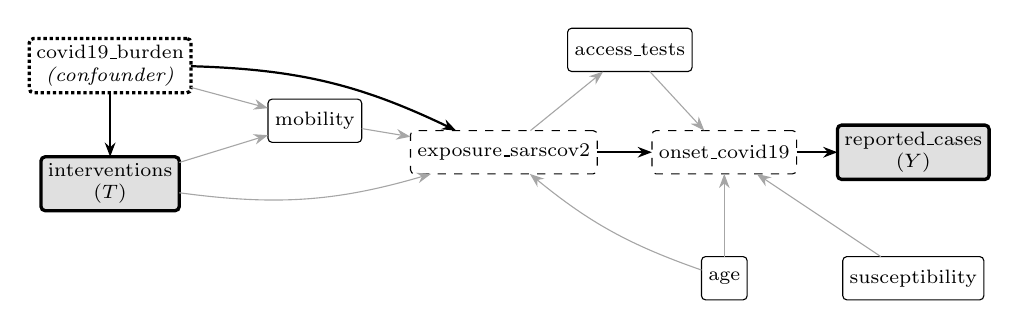
\begin{tikzpicture}[
    font=\scriptsize,
    >={Stealth[length=1.8mm]},
    node distance=6mm,
    obs/.style={draw, rounded corners=1.5pt, minimum height=5.5mm,
                inner sep=2.5pt, align=center, fill=white},
    lat/.style={draw, dashed, rounded corners=1.5pt, minimum height=5.5mm,
                inner sep=2.5pt, align=center, fill=white},
    tnode/.style={obs, fill=black!12, very thick},
    ynode/.style={obs, fill=black!12, very thick},
    conf/.style={obs, draw=black, densely dotted, very thick},
    edge/.style={->, gray!70},
    bd/.style={->, thick},               % backdoor-path edge
    every node/.style={outer sep=0pt}
]

% --- nodes (placed by topological flow, left -> right) ---
\node[conf]  (burden) at (0.0, 1.5)  {covid19\_burden \\ \textit{(confounder)}};
\node[tnode] (interv) at (0.0, 0.0)  {interventions \\ ($T$)};
\node[obs]   (mob)    at (2.6, 0.8)  {mobility};
\node[lat]   (exp)    at (5.0, 0.4)  {exposure\_sarscov2};
\node[obs]   (acc)    at (6.6, 1.7)  {access\_tests};
\node[obs]   (age)    at (7.8, -1.2) {age};
\node[obs]   (sus)    at (10.2, -1.2){susceptibility};
\node[lat]   (onset)  at (7.8, 0.4)  {onset\_covid19};
\node[ynode] (rep)    at (10.2, 0.4) {reported\_cases \\ ($Y$)};

% --- causal edges ---
\draw[edge] (interv) -- (mob);
\draw[edge] (burden) -- (mob);
\draw[edge] (mob)    -- (exp);
\draw[edge] (exp)    -- (acc);
\draw[edge] (acc)    -- (onset);
\draw[edge] (age)    -- (onset);
\draw[edge] (age)    to[bend left=10] (exp);
\draw[edge] (sus)    -- (onset);

% --- backdoor path: T <- burden -> exposure -> onset -> reported ---
\draw[bd] (burden) -- (interv);
\draw[bd] (burden) to[bend left=12] (exp);
\draw[edge] (interv) to[bend right=12] (exp);
\draw[bd] (exp)    -- (onset);
\draw[bd] (onset)  -- (rep);

\end{tikzpicture}

    \caption{A fragment of the COVID-19 causal DAG of Steiger et
    al.~\cite{steiger2021covid} used as running example. Solid boxes are
    observed variables, dashed boxes are latent ones. \textit{interventions}
    ($T$) and \textit{reported\_cases} ($Y$) are the treatment and the outcome
    of the queries of Section~\ref{sec:intro}; \textit{covid19\_burden} is a
    common cause of both and opens the backdoor path drawn in bold.}
    \label{fig:example}
\end{figure*}

Fig.~\ref{fig:example} shows a fragment of a COVID-19 causal DAG curated by
epidemiologists~\cite{steiger2021covid}, stored as a property graph, on
which we consider three situations. (a) An analyst asks for the confounders
of \textit{interventions} and \textit{reported\_cases}: the answer,
\textit{covid19\_burden}, is the intersection of two ancestor sets, a query a
graph database can answer only with two variable-length path traversals
followed by a client-side intersection. (b) The analyst asks whether
\textit{susceptibility} is independent of \textit{age} given
\textit{reported\_cases}: the two variables share no ancestor and are
independent, but conditioning on \textit{reported\_cases}, a descendant of the
collider \textit{onset\_covid19}, opens the path between them, so the answer
depends on edge orientation and on the conditioning set, which no path pattern
expresses. (c) A curator adds an edge from \textit{access\_tests} to
\textit{reported\_cases} as new evidence accrues: every ancestor set computed
so far for \textit{reported\_cases} is stale, and an external tool has no way
to know it.

Based on the above observations, one can notice a gap between what the store
offers and what the workload needs. Three difficulties stand in the way of
closing it, and none is solved by wrapping a library behind a stored
procedure. First, the operators are not all plain reachability: d-separation
and adjustment-set construction depend on the conditioning set and on edge
orientation, and require a conditioning-aware traversal rather than a
transitive closure. Second, answered by traversing the stored graph on every
call, each query costs $O(|V|+|E|)$, and identification issues many such
queries, so per-query traversal does not scale to large DAGs or high query
volume. Third, the structure that accelerates these queries must survive
updates: a causal graph under active curation cannot afford a full
recompilation after every edit.

A key requirement for any solution is therefore a representation of the DAG
from which whole ancestor and descendant sets, not only point-to-point
reachability, can be read in constant or near-constant time, because every
operator in the causal catalog (confounders, mediators, the forbidden set of
an adjustment problem, the canonical adjustment set) is an algebraic
combination of such sets. Precomputed reachability closures stored as bitsets
meet this requirement: a closure is one array read, an intersection is one
word-parallel operation, and the linear-time identification algorithms of
van der Zander et al.~\cite{vanderzander2019separators} consume exactly these
sets. We therefore build the index around them and design the query
processing and the maintenance around what they make cheap.

We present \textbf{Causal4j}, a system that makes causal structural queries a
native, indexed workload inside a property-graph DBMS (Neo4j). Causal4j has
three parts, shown in Fig.~\ref{fig:arch}: a declarative causal query language
whose statements compile to physical operators over the graph store, a
compiled causal index that snapshots the stored DAG into a dense layout with
precomputed ancestor and descendant bitsets, and an incremental maintenance
scheme that keeps the index consistent as the graph is edited. In sum, we make
the following contributions.
\begin{itemize}
  \item We propose a declarative causal query language embedded in a graph
  DBMS, covering reachability, path roles, independence, identification, and a
  quantitative layer, together with its compilation from language operators to
  Cypher writes and physical procedures (Section~\ref{sec:lang}).
  \item We introduce a compiled reachability index for causal DAGs (dense CSR
  adjacency, topological layers, and ancestor/descendant bitsets) and the
  query-processing algorithms built on it: bitset algebra for reachability and
  path roles, ancestral masking for d-separation, and identification by
  covariate adjustment through the constructive criterion and polynomial-delay
  enumeration of minimal adjustment sets (Section~\ref{sec:index}).
  \item We formalize incremental maintenance of the index under edge and
  variable mutations, with an insertion patch and a deletion recompute both
  bounded by the affected cone of the graph, and we use the same machinery to
  derive interventional worlds by graph surgery (Section~\ref{sec:incr}).
  \item We evaluate Causal4j on standard Bayesian-network DAGs and synthetic
  DAGs against in-DBMS traversal, Cypher, Neo4j GDS, and external causal
  libraries. The results show that \TODO{headline: $N\times$ lower latency on
  identification, index build under $X$~ms, incremental update $Y$ against
  $Z$ for recompilation, exact agreement with dagitty on every verdict}
  (Section~\ref{sec:eval}).
\end{itemize}

\begin{figure}[t]
    \centering
    \resizebox{\linewidth}{!}{%% ============================================================================
%% Figure: Causal4j architecture / query pipeline
%% Included from sections/introduction.tex (or main.tex) inside a figure env.
%% Requires in main.tex preamble:
%%   \usepackage{tikz}
%%   \usetikzlibrary{arrows.meta,positioning,fit,backgrounds}
%% Single-column figure. For a wide (two-column) version, wrap the caller in
%% figure* and bump node distances.
%% ============================================================================
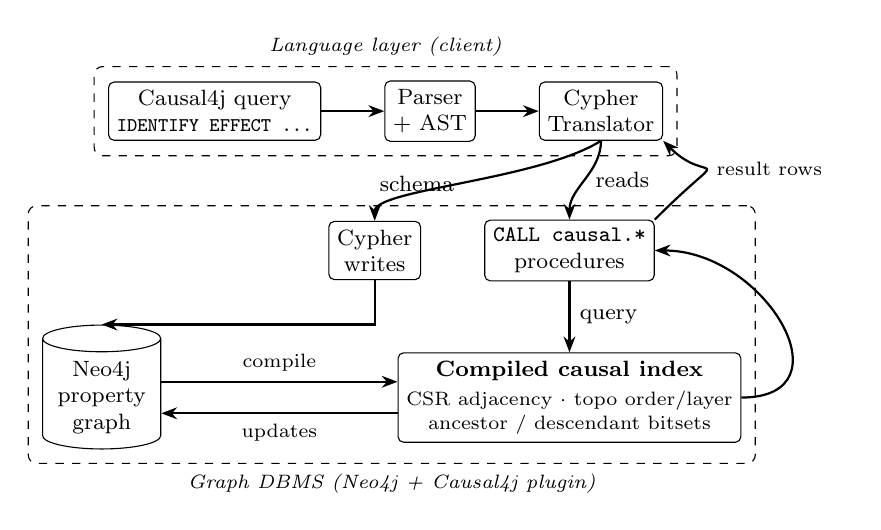
\begin{tikzpicture}[
    font=\footnotesize,
    >={Stealth[length=2mm]},
    box/.style={draw, rounded corners=2pt, align=center,
                minimum height=7mm, inner sep=3pt, fill=white},
    store/.style={draw, cylinder, shape border rotate=90, aspect=0.25,
                  align=center, minimum height=11mm, minimum width=15mm, fill=white},
    grp/.style={draw, dashed, rounded corners=3pt, inner sep=5pt},
    flow/.style={->, thick},
    node distance=5mm and 8mm
]

% --- language front-end ---
\node[box] (query) {Causal4j query \\ \texttt{\scriptsize IDENTIFY EFFECT ...}};
\node[box, right=of query] (ast) {Parser \\ + AST};
\node[box, right=of ast]  (trans) {Cypher \\ Translator};

\draw[flow] (query) -- (ast);
\draw[flow] (ast)   -- (trans);

% --- DBMS side ---
\node[box, below=10mm of trans, xshift=-4mm] (proc) {\texttt{CALL causal.*} \\ procedures};
\node[box, left=of proc] (writes) {Cypher \\ writes};

\draw[flow] (trans.south) .. controls +(0,-4mm) and +(0,4mm) .. (proc.north)
    node[midway, right] {reads};
\draw[flow] (trans.south) .. controls +(-8mm,-5mm) and +(0,4mm) .. (writes.north)
    node[midway, left] {schema};

% --- runtime / index ---
\node[box, below=9mm of proc, align=center] (index)
    {\textbf{Compiled causal index} \\[1pt]
     \scriptsize CSR adjacency $\cdot$ topo order/layer \\[-1pt]
     \scriptsize ancestor / descendant bitsets};
\node[store, left=30mm of index] (neo)
    {Neo4j \\ property \\ graph};

\draw[flow] (proc) -- (index) node[midway, right] {query};
\draw[flow] (writes.south) |- (neo.north) node[pos=0.75, above] {};
\draw[flow] ([yshift= 2mm]neo.east) -- ([yshift= 2mm]index.west)
    node[midway, above, font=\scriptsize] {compile};
\draw[flow] ([yshift=-2mm]index.west) -- ([yshift=-2mm]neo.east)
    node[midway, below, font=\scriptsize] {updates};

% --- results back to caller ---
\draw[flow] (index.east) .. controls +(14mm,0) and +(14mm,0) .. (proc.east);
\draw[flow] (proc.north east) .. controls +(10mm,10mm) and +(6mm,-6mm) .. (trans.south east)
    node[pos=0.5, right] {\scriptsize result rows};

% --- grouping boxes ---
\begin{scope}[on background layer]
  \node[grp, fit=(query)(ast)(trans), label={[font=\scriptsize\itshape]above:Language layer (client)}] {};
  \node[grp, fit=(writes)(proc)(index)(neo),
        label={[font=\scriptsize\itshape]below:Graph DBMS (Neo4j + Causal4j plugin)}] {};
\end{scope}

\end{tikzpicture}}
    \caption{Causal4j architecture. A statement is parsed and compiled into
    Cypher writes (definitions) or calls to \texttt{causal.*} procedures
    (queries); the procedures read a compiled snapshot of the stored DAG held
    by the plugin, which a transaction listener keeps consistent under
    updates.}
    \label{fig:arch}
\end{figure}

The remainder of the paper is structured as follows.
Section~\ref{sec:bg} defines causal DAGs, the query catalog, and the problem.
Section~\ref{sec:lang} presents the language and its compilation, and
Section~\ref{sec:compile} the compilation of the stored graph into a snapshot.
Section~\ref{sec:index} presents the index and the query-processing
algorithms, Section~\ref{sec:incr} incremental maintenance, and
Section~\ref{sec:quant} the quantitative layer. Section~\ref{sec:eval} reports
the experimental evaluation and Section~\ref{sec:related} discusses related
work. Finally, Section~\ref{sec:conclusion} concludes the paper.

%% ============================================================================
%% Section: Background and Problem
%% ============================================================================
\section{Background and Problem Statement}\label{sec:bg}

In this section, we introduce the preliminary notions needed as basic
ingredients in our framework: causal DAGs and their property-graph encoding,
the catalog of structural queries, and the data-engineering problem we
address.

\subsection{Causal DAGs and their property-graph encoding}\label{sec:bg:dag}

\begin{definition}[Causal DAG]
A causal DAG is a directed acyclic graph $G=(V,E)$ where $V$ is a set of
random variables and $E \subseteq V \times V$ is a set of edges such that
$X \rightarrow Y \in E$ asserts that $X$ is a direct cause of $Y$ relative to
the other variables in $V$~\cite{pearl2009causality}. A function
$\lambda: V \rightarrow \{\textit{observed}, \textit{latent}\}$ assigns to
each variable whether it is measured.
\end{definition}

Latent variables are retained in the model because they change which
conditional independencies hold and which effects are identifiable, even
though no data is ever assigned to them. We write $\pa(X)$, $\ch(X)$, $\an(X)$,
and $\de(X)$ for the parents, children, ancestors, and descendants of $X$;
ancestors and descendants are the transitive closures of parents and children
and exclude $X$ itself. For instance, in Fig.~\ref{fig:example}
$\pa(\textit{onset\_covid19}) = \{\textit{exposure\_sarscov2},
\textit{access\_tests}, \textit{age}, \textit{susceptibility}\}$ and
$\an(\textit{reported\_cases})$ contains every drawn variable except
\textit{reported\_cases} itself.

\noindent\textbf{Property-graph encoding.} Causal4j stores the DAG as a native
property graph. Each variable is a node
$(:\textsf{Variable}\;\{\textsf{id},\ \textsf{name},\ \textsf{observed},\ \textsf{latent}\})$
and each direct cause is a relationship
$(:\textsf{Variable})\text{-}[:\textsf{CAUSES}\;\{\textsf{active},\ \textsf{weight}\}]\!\rightarrow\!(:\textsf{Variable})$.
The \textsf{id} property is the canonical key; \textsf{active} lets a curator
toggle an edge without deleting it, and only edges with
$\textsf{active}=\text{true}$ participate in the model; \textsf{weight}
carries an optional structural coefficient used by the quantitative layer
(Section~\ref{sec:quant}) and ignored by the structural queries. This
encoding keeps the causal model in the database, co-located and jointly
queryable with any other graph data, rather than in a transient in-memory
object owned by an external tool.

\subsection{The causal query catalog}\label{sec:bg:catalog}

Analysts interrogate the DAG through a small and well-established catalog of
structural queries, which we group by the reasoning they support.

\noindent\textbf{Reachability queries} return $\pa$, $\ch$, $\an$, and $\de$
of a variable, and test whether a directed path $X \rightarrow \cdots
\rightarrow Y$ exists. They underpin every other query.

\noindent\textbf{Path-role queries} classify the variables that lie between a
treatment $T$ and an outcome $Y$. A \textit{mediator} lies on a directed path
$T \rightarrow \cdots \rightarrow Y$, i.e., it belongs to
$\de(T) \cap \an(Y)$; a \textit{confounder} is a common cause,
i.e., a variable in $\an(T) \cap \an(Y)$; a \textit{collider} between $X$ and
$Y$ is a variable $Z \notin \an(X) \cup \an(Y)$ with one parent in
$\de(X) \cup \{X\}$ and one parent in $\de(Y) \cup \{Y\}$, i.e., a variable
at which a path from $X$ and a path from $Y$ meet head to head. In
Fig.~\ref{fig:example}, \textit{covid19\_burden} is a confounder of
$T$ and $Y$, \textit{exposure\_sarscov2} and \textit{onset\_covid19} are
mediators, and \textit{onset\_covid19} is a collider between \textit{age} and
\textit{susceptibility}.

\noindent\textbf{Independence queries} test d-separation.

\begin{definition}[d-separation]
Let $X, Y \in V$ and $Z \subseteq V \setminus \{X,Y\}$. A path between $X$ and
$Y$ is blocked by $Z$ if it contains a non-collider that belongs to $Z$, or a
collider such that neither the collider nor any of its descendants belongs to
$Z$. $X$ and $Y$ are d-separated given $Z$, written $X \dsep Y \mid Z$, if
every path between them is blocked by $Z$~\cite{pearl2009causality}.
\end{definition}

D-separation is the graphical criterion for conditional independence and is
not plain reachability: adding a variable to $Z$ can block one path and, when
that variable is a collider or one of its descendants, open another. In
Fig.~\ref{fig:example}, $\textit{age} \dsep \textit{susceptibility} \mid
\emptyset$ holds, while conditioning on \textit{reported\_cases} opens the
path through the collider \textit{onset\_covid19}.

\noindent\textbf{Identification queries} decide whether the causal effect of
$T$ on $Y$ can be estimated from observational data by covariate adjustment
and, if so, return an adjustment set. We adopt the generalized adjustment
criterion~\cite{shpitser2010validity,perkovic2018complete}, which is complete
for DAGs and is the criterion implemented by reference
tools~\cite{textor2016dagitty}.

\begin{definition}[Adjustment criterion]
Let $T, Y \in V$ with $Y \in \de(T)$. The causal nodes are
$\cn(T,Y) = (\de(T) \cap \an(Y)) \cup \{Y\}$, i.e., the non-treatment
variables on directed paths from $T$ to $Y$, and the forbidden set is
$\forb(T,Y) = \de(\cn(T,Y)) \cup \cn(T,Y) \cup \{T\}$. The proper backdoor
graph $G^{\mathit{pbd}}_{T,Y}$ is $G$ without the edges $T \rightarrow C$ for
$C \in \cn(T,Y)$. A set $Z \subseteq V$ satisfies the adjustment criterion
relative to $(T,Y)$ if $Z \cap \forb(T,Y) = \emptyset$ and
$T \dsep Y \mid Z$ holds in $G^{\mathit{pbd}}_{T,Y}$.
\end{definition}

The criterion has a constructive form that we exploit in
Section~\ref{sec:index}: the effect is identifiable by adjustment if and only
if the canonical set $\adj(T,Y) = \an(\{T,Y\}) \setminus (\forb(T,Y) \cup
\{T,Y\})$ satisfies the criterion~\cite{vanderzander2019separators}. In
Fig.~\ref{fig:example}, $\{\textit{covid19\_burden}\}$ satisfies the
criterion for $(\textit{interventions}, \textit{reported\_cases})$, while
\textit{mobility} is forbidden since it lies on a directed path from $T$ to
$Y$. Listing all inclusion-minimal sets that satisfy the criterion is the most
expensive query of the catalog, since each candidate is validated by a
d-separation test.

\subsection{Problem statement}\label{sec:bg:problem}

We target the following data-engineering problem: supporting the causal query
catalog as a first-class workload inside a graph DBMS. Concretely, a solution
has to meet four requirements.
\begin{itemize}
  \item \textbf{R1 (Expressiveness).} A declarative interface in which each
  catalog query is a single statement, close to how analysts phrase causal
  questions, that compiles to physical operators over the graph store.
  \item \textbf{R2 (Efficiency).} Structural queries answered without
  re-traversing the stored graph on every call, so that the reachability and
  path-role operators are sublinear in graph size and identification issues a
  bounded number of conditioning-aware traversals.
  \item \textbf{R3 (Correctness).} Results faithful to the graphical semantics
  above, in particular a conditioning-aware d-separation test and an
  adjustment criterion that is complete for DAGs.
  \item \textbf{R4 (Maintainability).} The accelerating structure kept
  consistent under edge and variable updates without full recomputation, since
  curated causal graphs change continually.
\end{itemize}
None of these is served by exporting the DAG to an external library: R2 and
R4 in particular are database concerns (indexing, query processing, and
incremental maintenance), which is why we address them inside the DBMS.

%% ============================================================================
%% Section: The Causal Query Language
%% Operator -> procedure mapping follows dsl/.../exec/CypherTranslator.java
%% and plugin/.../api/ProcedureNames.java (see CODE-PLAN.md, WP2 and WP4).
%% ============================================================================
\section{The Causal Query Language}\label{sec:lang}

Requirement R1 asks for a declarative interface in which each catalog query is
a single statement that compiles to physical operators over the graph store.
In this section we present the language: its surface
(Section~\ref{sec:lang:surface}), the mapping from each operator to the
physical operator that answers it (Section~\ref{sec:lang:compile},
Table~\ref{tab:operators}), the registry through which a database holds
several causal worlds (Section~\ref{sec:lang:registry}), and how a model
enters the store (Section~\ref{sec:lang:populate}). The physical operators
themselves are the subject of Section~\ref{sec:index}.

\subsection{Design and surface syntax}\label{sec:lang:surface}

The language is a small statement-oriented DSL. A program is a sequence of
statements of three kinds: \textit{definition} statements declare variables
and edges and thereby write the causal model into the graph;
\textit{structural} statements ask the catalog queries of
Section~\ref{sec:bg:catalog}; \textit{quantitative} statements express
interventions and counterfactuals over a parameterized model
(Section~\ref{sec:quant}). Two design choices follow from R1. First, an
operator names a causal concept rather than a traversal: an analyst writes
\lstinline[style=causaldsl]|CONFOUNDERS OF T AND Y| and not a path pattern, so
the statement reads as the question and its compilation is the system's
concern. Second, every statement refers to variables by their canonical
\textsf{id}, so a query is portable across any database holding a model with
those variables.

Definition statements come in a standalone and a block form. A bare
\lstinline[style=causaldsl]|DEFINE CAUSAL VARIABLE| introduces one variable
with its observation status, and a
\lstinline[style=causaldsl]|DEFINE CAUSAL DAG| block declares a model as a
set of edges, optionally carrying a structural coefficient per edge:

\begin{lstlisting}[style=causaldsl]
DEFINE CAUSAL DAG CovidModel {
  covid19_burden    -> interventions
  covid19_burden    -> exposure_sarscov2
  interventions     -> mobility
  mobility          -> exposure_sarscov2
  exposure_sarscov2 -> onset_covid19
  onset_covid19     -> reported_cases
}
\end{lstlisting}

\noindent
Against the model so defined, the structural questions of the running example
are each one statement:

\begin{lstlisting}[style=causaldsl]
CONFOUNDERS OF interventions AND reported_cases
BACKDOOR PATHS BETWEEN interventions AND reported_cases
IDENTIFY EFFECT OF interventions ON reported_cases
  RETURN ADJUSTMENT SETS EXPLAIN
\end{lstlisting}

\noindent
The first returns \textit{covid19\_burden}; the second returns the variables
on backdoor paths; the third decides identifiability by adjustment and, with
\lstinline[style=causaldsl]|RETURN ADJUSTMENT SETS|, lists the minimal
adjustment sets, the optional \lstinline[style=causaldsl]|EXPLAIN| attaching
the canonical set and the forbidden set as witnesses of the decision. The
reachability and path-role operators
(\lstinline[style=causaldsl]|CAUSES OF|, \lstinline[style=causaldsl]|EFFECTS OF|,
\lstinline[style=causaldsl]|ANCESTORS OF|, \lstinline[style=causaldsl]|DESCENDANTS OF|,
\lstinline[style=causaldsl]|MEDIATORS BETWEEN|, \lstinline[style=causaldsl]|COLLIDERS BETWEEN|)
follow the same one-statement-per-question shape. The full grammar is given in
ANTLR form in our repository; Table~\ref{tab:operators} lists the operators
that matter for what follows.

\subsection{Compilation to physical operators}\label{sec:lang:compile}

A statement is parsed to an AST and compiled, statement by statement, to one or
more Cypher units executed inside the DBMS. The compiler emits two kinds of
unit. A definition statement compiles to Cypher \textit{writes} that maintain
the schema of Section~\ref{sec:bg:dag}: a \lstinline[style=causaldsl]|DEFINE|
becomes a \texttt{MERGE} of the \textsf{Variable} nodes and \textsf{CAUSES}
edges it introduces (one batched \texttt{UNWIND} for the edge set), after
which the transaction listener of Section~\ref{sec:incr} brings the compiled
snapshot up to date. A structural statement compiles to a \textit{read}: a
\texttt{CALL} of the \texttt{causal.*} procedure that answers it, which
consults the snapshot rather than the stored graph. This two-target
compilation is what keeps the model in the database: the language holds no
copy of the graph, and the same snapshot serves every reader.

\begin{table*}[t]
  \centering
  \caption{Language operators, their graphical semantics, and the physical
  operator each compiles to. Reachability and path-role operators map to
  \texttt{causal.*} procedures over the compiled snapshot
  (Section~\ref{sec:index}); d-separation is exposed as \texttt{causal.dsep}
  and is the inner test of identification. Definition statements compile to
  Cypher writes; world statements resolve in the server-side registry.}
  \label{tab:operators}
  \small
  \setlength{\tabcolsep}{4pt}
  \begin{tabular}{@{}p{0.30\linewidth} p{0.34\linewidth} p{0.30\linewidth}@{}}
    \toprule
    \textbf{DSL statement} & \textbf{Graphical meaning} & \textbf{Physical operator} \\
    \midrule
    \multicolumn{3}{@{}l}{\textit{Definition and worlds}}\\
    \lstinline[style=causaldsl]|DEFINE ... DAG| & write or update the model & \texttt{MERGE} + listener patch \\
    \lstinline[style=causaldsl]|INTERVENE ON X| & $do(X)$: remove edges into $X$ & \texttt{causal.intervene} (derived snapshot) \\
    \lstinline[style=causaldsl]|USE MODEL| / \lstinline[style=causaldsl]|RESET| & select the active world & \texttt{causal.use} \\
    \addlinespace[2pt]
    \multicolumn{3}{@{}l}{\textit{Reachability}}\\
    \lstinline[style=causaldsl]|CAUSES OF X|       & $\pa(X)$ & \texttt{causal.parents} \\
    \lstinline[style=causaldsl]|EFFECTS OF X|      & $\ch(X)$ & \texttt{causal.children} \\
    \lstinline[style=causaldsl]|ANCESTORS OF X|    & $\an(X)$ & \texttt{causal.ancestors} \\
    \lstinline[style=causaldsl]|DESCENDANTS OF X|  & $\de(X)$ & \texttt{causal.descendants} \\
    \addlinespace[2pt]
    \multicolumn{3}{@{}l}{\textit{Path roles}}\\
    \lstinline[style=causaldsl]|MEDIATORS ...|   & $\de(T) \cap \an(Y)$ & \texttt{causal.mediators} \\
    \lstinline[style=causaldsl]|COLLIDERS ...|   & head-to-head meeting points & \texttt{causal.colliders} \\
    \lstinline[style=causaldsl]|CONFOUNDERS ...| & $\an(T) \cap \an(Y)$ & \texttt{causal.confounders} \\
    \lstinline[style=causaldsl]|BACKDOOR PATHS ...| & variables on backdoor paths & \texttt{causal.backdoorVariables} \\
    \addlinespace[2pt]
    \multicolumn{3}{@{}l}{\textit{Independence and identification}}\\
    (inner test) & $X \dsep Y \mid Z$ & \texttt{causal.dsep} \\
    \lstinline[style=causaldsl]|IDENTIFY EFFECT ...| & adjustment criterion, canonical set & \texttt{causal.adjustmentSets} (canonical) \\
    \lstinline[style=causaldsl]|... RETURN ADJUSTMENT SETS| & minimal adjustment sets & \texttt{causal.adjustmentSets} (minimal) \\
    \addlinespace[2pt]
    \multicolumn{3}{@{}l}{\textit{Quantitative}}\\
    \lstinline[style=causaldsl]|INTERVENE ... RETURN EFFECT| & interventional means, total effect & \texttt{causal.linear\allowbreak GaussianInference} \\
    \lstinline[style=causaldsl]|COUNTERFACTUAL ...| & abduction, action, prediction & \texttt{causal.counterfactual} \\
    \bottomrule
  \end{tabular}
\end{table*}

Structural operators map to procedures one-to-one. The reachability operators
compile to \texttt{causal.parents}, \texttt{causal.children},
\texttt{causal.ancestors}, and \texttt{causal.descendants}; the path-role
operators to \texttt{causal.mediators}, \texttt{causal.colliders},
\texttt{causal.confounders}, and \texttt{causal.backdoorVariables};
\lstinline[style=causaldsl]|IDENTIFY EFFECT| compiles to
\texttt{causal.adjustmentSets}, whose mode argument selects the canonical set
(decision only) or the enumeration of minimal sets. D-separation is not a
top-level keyword but the inner test that identification issues; it is exposed
as \texttt{causal.dsep} so that the cost of the traversal-intensive part of
the workload is borne by one physical operator rather than by client-side
orchestration. The quantitative statements compile to
\texttt{causal.linearGaussianInference} and \texttt{causal.counterfactual}
(Section~\ref{sec:quant}).

\subsection{Model registry and causal worlds}\label{sec:lang:registry}

A causal database is rarely a single fixed graph: a curator maintains several
models, and an intervention $do(X)$ defines a derived model, the same DAG with
the edges into $X$ removed, that an analyst wants to name, query, and compare
against the original. The language therefore addresses models by name.
\lstinline[style=causaldsl]|DEFINE MODEL| registers a base model,
\lstinline[style=causaldsl]|USE MODEL| makes a named model (base or derived)
the active one, and \lstinline[style=causaldsl]|RESET| returns to the base
model while leaving derived worlds addressable. Every read procedure accepts
the model name as an optional argument, and the registry of named snapshots
lives in the plugin (Section~\ref{sec:compile}), so that switching worlds is
a name lookup on the server and a derived world is materialized once, by the
graph surgery of Section~\ref{sec:incr:worlds}, and shared by every later
statement that names it.

\subsection{Populating the store}\label{sec:lang:populate}

Definition statements are how a model enters the database, whether typed by
a curator or produced upstream. Everything statistical (structure discovery,
fitting of structural equations, refutation) is by design outside the DBMS:
an accompanying Python pipeline, built on causal-learn and DoWhy, discovers or
accepts a DAG, fits a linear-Gaussian model when requested, and emits a
grammar-valid program of definition statements with a provenance record. The
database receives only the finished structural artifact and performs graph
operations over it. This boundary is what makes the following sections a
database problem rather than a learning problem.

%% ============================================================================
%% Section: Compilation -- The Causal Snapshot
%% Faithful to GraphLoader.java, TopologicalSorter.java, CompiledCausalGraph.java,
%% RuntimeRegistry.java, DefaultCausalGraphRuntime.java (after WP1 and WP4).
%% ============================================================================
\section{Compilation: The Causal Snapshot}\label{sec:compile}

Structural queries are not answered against the stored property graph
directly. On \texttt{causal.compile} the graph is read once and compiled into
an immutable in-memory snapshot that every subsequent query reads. Compilation
is the boundary between the mutable, transactional graph and the
read-optimized structure of Section~\ref{sec:index}: it is where the
$O(|V|+|E|)$ scan is paid once, so that queries need not pay it again.

\noindent\textbf{Loading.} The loader performs two passes inside one read
transaction. The first pass materializes every \textsf{Variable} node with its
\textsf{observed}/\textsf{latent} flag and, when present, its linear-Gaussian
parameters; undeclared properties fall back to defaults. The second pass reads
the \textsf{CAUSES} relationships with a Cypher query that filters on
\lstinline[style=causaldsl]|coalesce(r.active, true)|, so only active edges
enter the snapshot and a curator can toggle an edge in or out of the model
without deleting it. Filtering in Cypher lets the DBMS use its own
relationship access rather than a full relationship scan in the plugin.

\noindent\textbf{Topological order and acyclicity.} The loader then computes
a topological order of the variables with Kahn's algorithm over the forward
adjacency. This serves two purposes: it is the order in which the closures of
Section~\ref{sec:index} and the recursions of Section~\ref{sec:quant} are
filled, and it is the acyclicity check. If the order fails to cover every
variable the graph contains a directed cycle and is not a DAG, and compilation
aborts with an error rather than admitting an ill-formed model. Enforcing the
DAG invariant at compile time (and at commit time, Section~\ref{sec:incr})
means that no downstream operator has to defend against cycles.

\noindent\textbf{The immutable snapshot.} The result is a compiled causal
graph: variables, forward and reverse adjacency, the topological order, the
closures of Section~\ref{sec:index}, and the SEM parameters, all held in
arrays that are never modified after construction. Immutability is deliberate.
Since the snapshot never changes, every reader sees a consistent view without
locking, and the index can be built once and cached rather than reconstructed
per query. The snapshot is also the single source of truth: derived facts
(ancestors, adjustment sets) are exposed through \texttt{causal.*} procedures
over it rather than materialized back into the graph as extra relationships,
which would double the maintenance burden under updates.

\noindent\textbf{Runtime registry and consistency.} Neo4j instantiates a
procedure class afresh for every call, so the snapshot cannot live inside a
procedure. It is held instead by a process-scoped registry that maps a model
name to a runtime owning the current snapshot of that model in a single
\texttt{volatile} reference. Recompilation, incremental patching, and
invalidation are serialized per model, while all reads are lock-free: a query
captures the current reference once and works against that fixed snapshot,
so a concurrent recompile or patch installs a new snapshot without exposing a
partially built one. This gives a snapshot-isolated consistency model: a
query runs entirely against the model as of the compile or patch that
produced its snapshot. When and how a new snapshot is installed, by full
recompilation or by the incremental patch that avoids re-reading the graph,
is the subject of Section~\ref{sec:incr}.

%% ============================================================================
%% Section: Indexing and Query Processing (CORE)
%% Owns Table tab:complexity and Fig fig:index.
%% Design follows CODE-PLAN.md WP1 (layout, closures) and WP2 (algorithms).
%% ============================================================================
\section{Indexing and Query Processing}\label{sec:index}

This section is the core of the paper. We present the physical layout the
snapshot compiles to (Section~\ref{sec:index:layout}), the precomputed
reachability closures that accelerate every structural query
(Section~\ref{sec:index:bitsets}), and the query-processing algorithms built
on them: reachability and path roles (Section~\ref{sec:index:reach}),
conditioning-aware d-separation (Section~\ref{sec:index:dsep}), and
identification by adjustment (Section~\ref{sec:index:adj}).
Table~\ref{tab:complexity} summarizes the per-operator cost against a
map-of-sets baseline, distinguishing the operators that become sublinear from
those that keep a linear traversal with a smaller constant.

\subsection{Physical layout}\label{sec:index:layout}

The snapshot's variables are assigned dense integer indices $0..n-1$ through a
\textsf{name}$\to$\textsf{index} map, so that every downstream structure is an
array rather than a hash map (Fig.~\ref{fig:index}). Edges are stored as
compressed sparse rows: a forward and a reverse offset/target array pair, so
that the children of $i$ are the slice
$\textsf{fwdTarget}[\textsf{fwdOffset}[i] .. \textsf{fwdOffset}[i{+}1])$ and
the parents of $i$ the symmetric slice of the reverse pair, giving
cache-friendly, allocation-free neighbor iteration. The topological order is
stored as an \texttt{int[]} together with its inverse, and each node carries
its layer $\textsf{layer}[i]$ (0 for sources, otherwise one more than the
maximum layer of its parents), which lets a traversal prune any neighbor that
cannot lie on a path between two nodes by a layer comparison. This replaces
the baseline representation, a \lstinline[style=causaldsl]|Map<String,Set<String>>|
adjacency with string-keyed lookups and per-query depth-first search, whose
every structural query costs an $O(|V|+|E|)$ traversal with hashing and
boxing overhead.

\subsection{Reachability closures as bitsets}\label{sec:index:bitsets}

On top of the dense layout we precompute, for every variable, its ancestor set
and its descendant set as fixed-width bitsets
$\textsf{anc}[i], \textsf{des}[i] \in \{0,1\}^n$ packed into
$w = \lceil n/64 \rceil$ machine words. The ancestor closures are filled in a
single forward-topological sweep with the recurrence
\[
  \textsf{anc}[i] \;=\; \bigcup_{p \in \pa(i)} \bigl(\textsf{anc}[p] \cup \{p\}\bigr),
\]
and the descendant closures symmetrically in reverse-topological order. Each
sweep performs one word-parallel union per edge, so the build costs
$O((|V|+|E|)\, w)$ time and the two closures occupy $2\,|V|\,w$ words of
space, i.e., $O(|V|^2/64)$. This is a deliberate space-for-time trade: it
turns reachability from a traversal into a bit test and, more importantly for
the causal workload, delivers whole ancestor and descendant sets as single
array reads. We discuss when the trade stops paying at the end of this
section.

\begin{figure}[t]\centering
  \resizebox{\linewidth}{!}{%% ============================================================================
%% Figure: compiled index layout (dense CSR + reachability bitsets)
%% Included from sections/indexing.tex inside a figure env via \resizebox{\input}.
%% Requires: \usepackage{tikz}; \usetikzlibrary{positioning,fit}
%% Example DAG: A(0)->B(1), A(0)->C(2), B(1)->D(3), C(2)->D(3)
%% ============================================================================
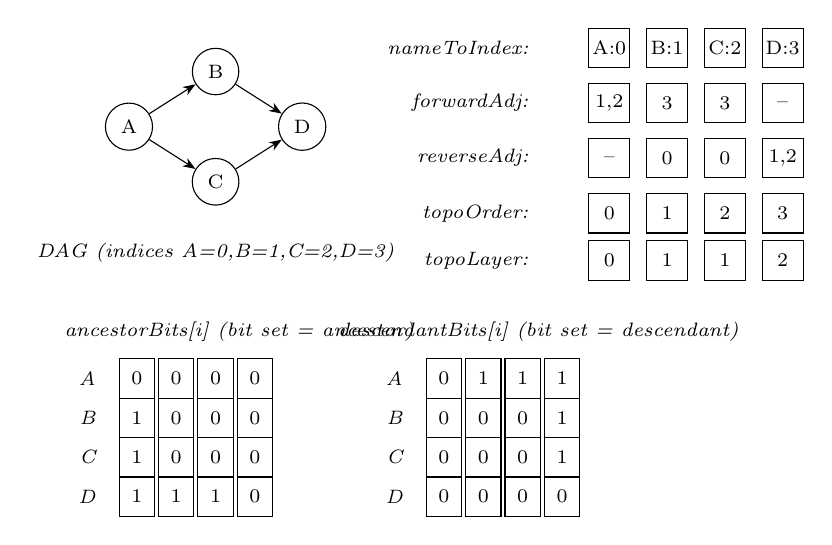
\begin{tikzpicture}[
    font=\scriptsize,
    >={Stealth[length=1.6mm]},
    cell/.style={draw, minimum width=5.2mm, minimum height=5mm, inner sep=1pt,
                 align=center, fill=white},
    lab/.style={anchor=east, font=\scriptsize\itshape},
    node distance=2mm,
]

% ---- tiny example DAG (top-left) ----
\node[draw, circle, minimum size=5mm] (A) at (0,0)      {A};
\node[draw, circle, minimum size=5mm] (B) at (1.1,0.7)  {B};
\node[draw, circle, minimum size=5mm] (C) at (1.1,-0.7) {C};
\node[draw, circle, minimum size=5mm] (D) at (2.2,0)    {D};
\draw[->] (A) -- (B); \draw[->] (A) -- (C);
\draw[->] (B) -- (D); \draw[->] (C) -- (D);
\node[font=\scriptsize\itshape] at (1.1,-1.6) {DAG (indices A{=}0,B{=}1,C{=}2,D{=}3)};

% ---- name -> index map ----
\node[lab] (m0) at (5.2, 1.0) {nameToIndex:};
\node[cell] (mA) at (6.1,1.0) {A:0};
\node[cell, right=of mA] (mB) {B:1};
\node[cell, right=of mB] (mC) {C:2};
\node[cell, right=of mC] (mD) {D:3};

% ---- forward CSR ----
\node[lab] (f0) at (5.2, 0.3) {forwardAdj:};
\node[cell] (f1) at (6.1,0.3) {1,2};
\node[cell, right=of f1] (f2) {3};
\node[cell, right=of f2] (f3) {3};
\node[cell, right=of f3] (f4) {--};

% ---- reverse CSR ----
\node[lab] (r0) at (5.2, -0.4) {reverseAdj:};
\node[cell] (r1) at (6.1,-0.4) {--};
\node[cell, right=of r1] (r2) {0};
\node[cell, right=of r2] (r3) {0};
\node[cell, right=of r3] (r4) {1,2};

% ---- topo order / layer ----
\node[lab] (t0) at (5.2, -1.1) {topoOrder:};
\node[cell] (t1) at (6.1,-1.1) {0};
\node[cell, right=of t1] (t2) {1};
\node[cell, right=of t2] (t3) {2};
\node[cell, right=of t3] (t4) {3};
\node[lab] (l0) at (5.2, -1.7) {topoLayer:};
\node[cell] (l1) at (6.1,-1.7) {0};
\node[cell, right=of l1] (l2) {1};
\node[cell, right=of l2] (l3) {1};
\node[cell, right=of l3] (l4) {2};

% ---- ancestor bitsets (rows = variable, columns = bit for A B C D) ----
\node[font=\scriptsize\itshape] at (1.4,-2.6) {ancestorBits[i] (bit set = ancestor)};
\node[lab] at (-0.3,-3.2) {A}; \node[lab] at (-0.3,-3.7) {B};
\node[lab] at (-0.3,-4.2) {C}; \node[lab] at (-0.3,-4.7) {D};
% rows explicitly (A,B,C,D) x (A,B,C,D)
\foreach \row/\y/\vals in {A/-3.2/{0/0,1/0,2/0,3/0}, B/-3.7/{0/1,1/0,2/0,3/0},
                           C/-4.2/{0/1,1/0,2/0,3/0}, D/-4.7/{0/1,1/1,2/1,3/0}} {
  \foreach \c/\v in \vals {
    \node[cell, minimum width=4.5mm] at ({0.1+\c*0.5},\y) {\v};
  }
}

% ---- descendant bitsets ----
\node[font=\scriptsize\itshape] at (5.2,-2.6) {descendantBits[i] (bit set = descendant)};
\node[lab] at (3.6,-3.2) {A}; \node[lab] at (3.6,-3.7) {B};
\node[lab] at (3.6,-4.2) {C}; \node[lab] at (3.6,-4.7) {D};
\foreach \row/\y/\vals in {A/-3.2/{0/0,1/1,2/1,3/1}, B/-3.7/{0/0,1/0,2/0,3/1},
                           C/-4.2/{0/0,1/0,2/0,3/1}, D/-4.7/{0/0,1/0,2/0,3/0}} {
  \foreach \c/\v in \vals {
    \node[cell, minimum width=4.5mm] at ({4.0+\c*0.5},\y) {\v};
  }
}

\end{tikzpicture}
}
  \caption{Compiled index layout for a small fragment. Variables map to dense
  indices; forward and reverse CSR arrays store adjacency; a topological order
  and a per-node layer drive pruning; per-node ancestor and descendant bitsets
  ($\lceil n/64\rceil$ words each) are filled in forward- and
  reverse-topological order.}
  \label{fig:index}
\end{figure}

\subsection{Reachability and path-role queries}\label{sec:index:reach}

With the closures in hand the reachability operators are immediate: $\an(X)$
and $\de(X)$ are one array read, and a directed path from $X$ to $Y$ exists if
and only if bit $Y$ is set in $\textsf{des}[X]$, an $O(1)$ test. The path-role
operators reduce to bitset algebra over the closures:
{\small
\begin{align*}
  \text{confounders}(T,Y) &= \textsf{anc}[T] \cap \textsf{anc}[Y], \\
  \text{mediators}(T,Y)   &= \textsf{des}[T] \cap \textsf{anc}[Y], \\
  \cn(T,Y)   &= \text{mediators}(T,Y) \cup \{Y\}, \\
  \forb(T,Y) &= \{T\} \cup \cn(T,Y) \cup \textstyle\bigcup_{C \in \cn(T,Y)} \textsf{des}[C], \\
  \adj(T,Y)  &= (\textsf{anc}[T] \cup \textsf{anc}[Y]) \\
             &\qquad \setminus (\forb(T,Y) \cup \{T,Y\}).
\end{align*}}
Each of the first three is $O(w)$ word operations; the forbidden set costs
one union per causal node, $O(|\cn(T,Y)|\, w)$, and the canonical set two
more word operations. Colliders between $X$ and $Y$ are the variables outside
$\textsf{anc}[X] \cup \textsf{anc}[Y]$ having one parent in
$\textsf{des}[X] \cup \{X\}$ and one in $\textsf{des}[Y] \cup \{Y\}$, which
is one bit test per parent of each candidate. The variables on backdoor paths
are found by a breadth-first search on the skeleton starting from $\pa(T)$
that never enters $\forb(T,Y)$, with the visited set as a bitset. In the
running example, $\text{confounders}(\textit{interventions},
\textit{reported\_cases})$ is a single intersection returning
\textit{covid19\_burden}, and $\forb$ contains \textit{mobility},
\textit{exposure\_sarscov2}, \textit{onset\_covid19}, and their descendants.

\subsection{Conditioning-aware d-separation}\label{sec:index:dsep}

D-separation is not reachability: adding a variable to the conditioning set
$Z$ can block one path and, when that variable is a collider or one of its
descendants, open another. The test must follow edge orientation and the role
of each node under $Z$, which we do with the Bayes-Ball
procedure~\cite{shachter1998bayesball}. A search propagates balls from $X$,
tracking for each visited node whether it was entered from a parent or from a
child; at each node the admissible continuations depend on whether the node is
in $Z$: a node in $Z$ entered from a parent bounces the ball back to its
parents and blocks it otherwise, while a node outside $Z$ passes a ball
entered from a parent to its children and a ball entered from a child to both
its parents and its children. $X$ and $Y$ are d-separated given $Z$ exactly
when no ball reaches $Y$. The procedure is conditioning-aware by construction
and visits each (node, direction) state at most once, so its cost is
$O(|V|+|E|)$ in the worst case. Bitsets do not change this bound. However,
they change the constant in two ways. First, $X$, $Y$, $Z$, the two visited
sets, and the set of nodes whose outgoing edges are cut are all bitsets, so
membership is one word test and the traversal allocates nothing. Second,
d-separation of $X$ and $Y$ given $Z$ depends only on the subgraph induced by
$\an(X \cup Y \cup Z) \cup X \cup Y \cup Z$~\cite{geiger1990identifying}, and
that set is one union of closures: the traversal is masked to it and never
enqueues a node outside, which on sparse DAGs with small $Z$ prunes most of
the graph. Section~\ref{sec:eval} measures the effect of masking separately
from the effect of the representation. A flag cutting the outgoing edges of
the treatment towards its causal nodes turns the same routine into the
separation test in the proper backdoor graph used next.

\subsection{Identification by adjustment}\label{sec:index:adj}

Identification asks whether the effect of $T$ on $Y$ is estimable by covariate
adjustment and, if so, for one or all minimal adjustment sets. A naive
approach enumerates candidate sets and validates each with a d-separation
test; since the number of candidates is exponential in $|V|$, no speed-up of
the inner test makes it scale. We instead build on the constructive results
of van der Zander et al.~\cite{vanderzander2014constructing,vanderzander2019separators},
whose steps consume exactly the sets the index stores.

\noindent\textbf{Decision.} The effect is identifiable by adjustment if and
only if the canonical set $\adj(T,Y)$ satisfies the adjustment criterion.
Since $\adj(T,Y)$ is disjoint from $\forb(T,Y)$ by construction, the decision
is one closure construction ($O(|\cn(T,Y)|\,w)$ word operations) followed by
one masked Bayes-Ball run in the proper backdoor graph. This is the default of
\lstinline[style=causaldsl]|IDENTIFY EFFECT|: a query with no open backdoor
path returns after a single traversal, and so does a query on a graph with
thousands of variables.

\noindent\textbf{Enumeration.} Minimal adjustment sets are minimal separators
of $T$ and $Y$ in the proper backdoor graph restricted to the allowed
variables $R = V \setminus (\forb(T,Y) \cup \{T,Y\})$. We implement the
separator framework of~\cite{vanderzander2019separators} in three routines.
(1) $\textsc{FindSep}(I,R)$ returns $\bigl(\an(\{T,Y\} \cup I) \cap R\bigr)
\setminus \{T,Y\}$ if that set separates $T$ and $Y$, and reports that no
separator containing $I$ within $R$ exists otherwise; the candidate is one
union of closures and the check one traversal.
(2) $\textsc{FindMinSep}(I,R)$ shrinks the result of \textsc{FindSep} to an
inclusion-minimal separator by two reachability passes in the moralized
ancestral graph of $T$, $Y$, and the candidate, keeping only the candidate
variables reachable from $T$ and then from $Y$; the ancestral graph is the
mask of the previous section and moralization is local to it.
(3) $\textsc{ListMinSep}(I,R)$ enumerates all minimal separators by
branching on one allowed variable $v$ at a time, either forcing it into $I$
or removing it from $R$, and pruning a branch as soon as \textsc{FindMinSep}
reports that no separator exists in it. Every leaf emits one minimal set and
every internal node performs a bounded number of closure unions and
traversals, so the enumeration runs with polynomial
delay~\cite{vanderzander2019separators}: the time between two consecutive
answers is polynomial in $|V|$ regardless of how many answers there are.
\lstinline[style=causaldsl]|RETURN ADJUSTMENT SETS| streams the result of
\textsc{ListMinSep} with an optional limit, and \textsc{FindMinSep} alone
answers a request for a single minimal set.

\begin{table}[t]\centering
\caption{Per-operator cost of the map-of-sets baseline with per-query DFS and
of the bitset index, with $w = \lceil |V|/64 \rceil$, $c = |\cn(T,Y)|$, and
$V_m, E_m$ the nodes and edges of the ancestral mask. Tier (a) operators are sublinear;
tier (b) keeps a linear traversal with bitset membership and ancestral
masking; tier (c) replaces exponential enumeration with a bounded number of
tier (a) and (b) steps per answer.}
\label{tab:complexity}
\footnotesize
\setlength{\tabcolsep}{3pt}
\begin{tabular}{@{}llll@{}}
\toprule
Operator & Baseline & Index & Tier \\
\midrule
ancestors / descendants & $O(|V|{+}|E|)$ & $O(w)$ & (a) \\
directed path test      & $O(|V|{+}|E|)$ & $O(1)$ & (a) \\
confounders / mediators & $O(|V|{+}|E|)$ & $O(w)$ & (a) \\
forbidden / canonical set & $O(c(|V|{+}|E|))$ & $O(c\,w)$ & (a) \\
colliders               & $O(|V|{+}|E|)$ & $O(|E|)$ bit tests & (a) \\
d-separation (masked)   & $O(|V|{+}|E|)$ & $O(|V_m|{+}|E_m|)$ & (b) \\
identifiability decision & $O(2^{|V|})$ tests & $O(c\,w)$ + 1 test & (c) \\
minimal sets (each)     & $O(2^{|V|})$ tests & poly. delay & (c) \\
\midrule
index space             & $O(|V|{+}|E|)$ & $O(|V|{+}|E| + |V|\,w)$ & \\
index build             & $O(|V|{+}|E|)$ & $O((|V|{+}|E|)\,w)$ & \\
\bottomrule
\end{tabular}
\end{table}

\noindent\textbf{When closures stop paying.} The closures cost $2|V|w$ words:
about 25~MB for $|V| = 10^4$ and about 2.5~GB for $|V| = 10^5$. For DAGs
beyond a configured memory budget the snapshot keeps only the CSR layout and
the layer array, and answers reachability by a layer-pruned depth-first search
that never follows a neighbor whose layer lies outside the interval between
the two endpoints; path-role and identification operators then run over
sets computed on demand, at the baseline cost of Table~\ref{tab:complexity}
minus the hashing overhead. The choice is made once at compile time from
$|V|$ and the budget, and Section~\ref{sec:eval} reports the latency and
memory of both branches so that the crossover is a measured quantity rather
than a guess. Causal DAGs curated by domain experts are, in our experience,
well below the crossover: the largest reference network we use has
$|V| = 1041$ and its closures fit in about 280~KB.

%% ============================================================================
%% Section: Incremental Index Maintenance
%% Follows CODE-PLAN.md WP3 (patch, cone recompute, flips, validation) and
%% WP4 (derived worlds by graph surgery).
%% ============================================================================
\section{Incremental Index Maintenance}\label{sec:incr}

A curated causal graph is edited continually: an edge is added as evidence
accrues, a variable is reclassified as latent, an edge is deactivated pending
review. Requirement R4 asks that the compiled index survive these edits
without a full recompilation after every change. In this section we describe
how Causal4j observes graph mutations, validates them, and patches the
snapshot within the region of the graph they affect.

\noindent\textbf{Observing and validating changes.} The plugin registers a
transaction-event listener, scoped to the database for its lifetime, that
sees every committing write. Before a transaction commits, the listener
inspects the transaction data and, if it touches the causal schema, distills
the change into a compact change batch: created and deleted \textsf{Variable}
nodes, created and deleted \textsf{CAUSES} edges, edges whose \textsf{active}
flag flipped (treated as insertions or deletions), and variables whose
\textsf{latent} flag flipped. Transactions that touch no \textsf{Variable}
node and no \textsf{CAUSES} edge are rejected by a guard on the transaction
data and cost nothing. The pre-commit hook is also where the DAG invariant is
enforced: for every inserted edge $u \rightarrow v$, the listener tests
whether $v$ reaches $u$ in the current closures or through the other edges of
the same batch, and aborts the transaction if so, so that an invalid model
never reaches the store. The batch is handed to the post-commit hook, which
applies it once the write is durable.

\noindent\textbf{Insertion patch.} Given a change batch, the closures of
Section~\ref{sec:index:bitsets} can be maintained locally rather than
rebuilt. Inserting an edge $u \rightarrow v$ extends the CSR adjacency and
propagates closures over the affected cone only: every node in
$\an(u) \cup \{u\}$ gains $\textsf{des}[v] \cup \{v\}$ as new descendants, and
every node in $\de(v) \cup \{v\}$ gains $\textsf{anc}[u] \cup \{u\}$ as new
ancestors. Both gains are one bitset each, read from the snapshot before the
patch, and each affected row receives one word-parallel union, so the patch
costs $(|\an(u)| + |\de(v)| + 2)\,w$ word operations. Layers are relabeled
for $v$ and its descendants only when $\textsf{layer}[v] \le
\textsf{layer}[u]$. Nodes outside the two cones are untouched.

\noindent\textbf{Deletion by cone recompute.} Deleting $u \rightarrow v$ can
shrink closures in a way that no local union expresses, since a node may
have lost one of several paths. However, the rows that can change are still
bounded: only the ancestor sets of $C = \de(v) \cup \{v\}$ and the descendant
sets of $C' = \an(u) \cup \{u\}$ pass through the deleted edge. We therefore
recompute $\textsf{anc}$ over $C$ in topological order from the updated
parents, and $\textsf{des}$ over $C'$ in reverse topological order from the
updated children, with the recurrence of Section~\ref{sec:index:bitsets}
restricted to those rows; rows outside $C \cup C'$ are provably unchanged.
The cost is $O((|C| + |C'| + |E_{C \cup C'}|)\,w)$, and full recompilation
remains the fallback when $|C| + |C'|$ exceeds a threshold, which
Section~\ref{sec:eval} measures. Adding a variable allocates a dense index
and, one time in 64, one more word per row; removing a variable deletes its
incident edges and frees its index. A \textsf{latent} flip is a property-only
update that leaves the closures untouched.

\noindent\textbf{Copy-on-write and consistency.} A patch never mutates the
snapshot that readers hold. It produces a new snapshot that shares every
untouched row and array with the old one and replaces the rows of the
affected cones, and it is published with a single reference store, exactly
as a recompile is. In this way the snapshot-isolated consistency model of
Section~\ref{sec:compile} is preserved without locks, and the memory cost of a
patch is proportional to the cone rather than to the graph. Batches are
applied by first recomputing the union of the deletion cones once and then
applying the insertion unions, so that a transaction with many edits costs
one cone recompute rather than one per edit.

\subsection{Derived worlds by graph surgery}\label{sec:incr:worlds}

An intervention $do(X)$ defines a derived model, the same DAG with the edges
into $X$ removed, and the language of Section~\ref{sec:lang:registry} lets an
analyst name such a world and query it. The deletion machinery above is
exactly what constructs it: \texttt{causal.intervene} applies a batch that
deletes the incoming edges of every intervened variable to a copy of the base
snapshot, recomputes the affected cones, and registers the result under the
world's name. Since the copy shares every untouched row with the base, a
derived world costs the cone recompute in time and the changed rows in
memory, and a later structural statement over it reads its own closures like
any other snapshot. The same mechanism gives \textit{what-if} structural
queries over hypothetical edits (a proposed edge, a removed confounder)
without touching the stored graph.

%% ============================================================================
%% Section: Quantitative Layer (kept short: expressiveness, not a contribution)
%% Faithful to LinearGaussianInference.java, CounterfactualInference.java.
%% ============================================================================
\section{Quantitative Layer}\label{sec:quant}

The same compiled snapshot that answers structural queries also carries
optional numeric parameters, which let Causal4j answer quantitative causal
questions (interventions and counterfactuals) without leaving the DBMS. We
describe the layer briefly: it is a demonstration of the expressiveness the
indexed engine enables, not a contribution of the paper.

\noindent\textbf{Linear-Gaussian model.} When a model is parameterized, each
variable follows the structural equation
$V = \mu_{0,V} + \sum_{P \in \pa(V)} \beta_{P \rightarrow V}\,P + \varepsilon_V$
with $\varepsilon_V \sim \mathcal{N}(0, \sigma^2_V)$, where the edge
coefficients $\beta$, intercepts $\mu_0$, and noise variances $\sigma^2$ are
the \textsf{weight}, \textsf{intercept}, and \textsf{noise} properties read at
compile time (Section~\ref{sec:compile}). The parameters are supplied by the
upstream pipeline of Section~\ref{sec:lang:populate} or by the curator; the
DBMS never fits them. The snapshot reports itself parameterized only when some
value departs from the structural-only defaults, so a purely qualitative DAG
incurs no numeric machinery.

\noindent\textbf{Interventions and counterfactuals.} The do-operator
$do(X{=}x)$ fixes the mean of $X$ to $x$, sets its variance to zero, and drops
its incoming edges, which the general recursion then handles with no special
case. Interventional means propagate in topological order,
$\mu(V) = \mu_{0,V} + \sum_P \beta_{P \rightarrow V}\,\mu(P)$; interventional
variances follow from a covariance recursion in the same order; and the total
effect of $T$ on $Y$ is obtained by unit-impulse propagation
($\partial T = 1$, $\partial V = \sum_P \beta_{P \rightarrow V}\,\partial P$,
read off at $Y$), avoiding any path enumeration. Counterfactuals follow the
abduction, action, and prediction recipe over the same equations: infer the
exogenous noise consistent with the observed factual world, apply the
hypothesized intervention, and re-propagate. Every step reuses the
topological order already on the snapshot, so the quantitative layer adds
semantics, not a second data structure. On a parameterized version of the
running example,
\lstinline[style=causaldsl]|INTERVENE ON interventions = 1 COMPARE TO interventions = 0 RETURN EFFECT ON reported_cases|
returns the total effect along the directed paths, while a
\lstinline[style=causaldsl]|COUNTERFACTUAL| statement answers what
\textit{reported\_cases} would have been for one observed unit under a
different intervention. Since $do(\cdot)$ also yields a derived structural
world (Section~\ref{sec:incr:worlds}), the qualitative and quantitative
layers close the loop over a single stored graph.

%% ============================================================================
%% Section: Evaluation
%% Owns Table tab:datasets, Table tab:coverage, Fig fig:latency, Fig fig:incr.
%% Design is final; every number is a \TODO until bench/run_all.sh (CODE-PLAN
%% WP5) produces paper/numbers.tex. Do not type numbers by hand.
%% ============================================================================
\section{Experimental Evaluation}\label{sec:eval}

In this section, we present an experimental evaluation to assess the
efficiency, the cost, and the correctness of Causal4j. We ask five questions.
\textbf{RQ1 (query performance):} how do structural and identification
queries compare in latency and throughput against in-DBMS and external
alternatives? \textbf{RQ2 (index cost):} what does the index cost to build
and to store as a function of graph size and density, and where is the
crossover with the layer-pruned branch? \textbf{RQ3 (maintenance):} when does
incremental maintenance beat full recompilation, and what does a mixed
workload of edits and queries observe? \textbf{RQ4 (scalability):} how does
latency grow with $|V|$? \textbf{RQ5 (correctness):} do the answers agree
with reference causal tools? All the material necessary to reproduce the
results, together with the hardware specifications, is available on our
online repository\footnote{\TODO{URL of the artifact.}}.

\noindent\textbf{Settings.} \TODO{Hardware (CPU, RAM), JVM version and heap,
Neo4j version (2025.x, embedded through the test harness and as a server for
the Cypher and GDS baselines), JMH configuration: 5 forks, 5 warm-up and 10
measurement iterations per operator; medians with interquartile ranges are
reported.} The index and the baseline share every line of code outside the
representation of the snapshot, so a difference in latency is attributable
to the representation and the algorithms of Section~\ref{sec:index} alone.

\noindent\textbf{Datasets.} We use three families of DAGs
(Table~\ref{tab:datasets}): (i) the reference Bayesian networks of the bnlearn
repository~\cite{scutari2010bnlearn}, taken as causal DAGs, from
\textsc{asia} to \textsc{munin}, which are recognized and reproducible and
span three orders of magnitude in $|V|$; (ii) synthetic DAGs generated by
orienting Erd\H{o}s-R\'enyi and preferential-attachment graphs along a
random vertex order, with $|V|$ from $10^2$ to $10^4$ and average degree in
$\{2, 4, 8\}$ controlled independently, five seeds each, which let us sweep
size and density separately; and (iii) the COVID-19 DAG of the running
example~\cite{steiger2021covid} with $25$ variables and $78$ edges. To
control the workload, every system receives the same $200$ random
treatment-outcome pairs $(T,Y)$ with $Y \in \de(T)$ and the same $200$
random triples $(X,Y,Z)$ with $|Z| \in \{0, 1, 3, 10\}$ per dataset.

\begin{table}[t]\centering
\caption{Datasets. \NOTE{Verify $|V|$ and $|E|$ against the bnlearn
repository before submission; closure memory is $2|V|\lceil|V|/64\rceil$
words.}}
\label{tab:datasets}
\footnotesize
\setlength{\tabcolsep}{3pt}
\begin{tabular}{@{}lrrrr@{}}
\toprule
DAG & $|V|$ & $|E|$ & longest path & closures \\
\midrule
\textsc{asia}       &    8 &    8 & \TODO{} & 128~B \\
\textsc{sachs}      &   11 &   17 & \TODO{} & 176~B \\
\textsc{child}      &   20 &   25 & \TODO{} & 320~B \\
\textsc{alarm}      &   37 &   46 & \TODO{} & 592~B \\
\textsc{hepar2}     &   70 &  123 & \TODO{} & 2.2~KB \\
\textsc{win95pts}   &   76 &  112 & \TODO{} & 2.4~KB \\
\textsc{pathfinder} &  109 &  195 & \TODO{} & 3.5~KB \\
\textsc{andes}      &  223 &  338 & \TODO{} & 14~KB \\
\textsc{pigs}       &  441 &  592 & \TODO{} & 49~KB \\
\textsc{link}       &  724 & 1125 & \TODO{} & 139~KB \\
\textsc{munin}      & 1041 & 1397 & \TODO{} & 283~KB \\
COVID-19            &   25 &   78 & \TODO{} & 400~B \\
synthetic           & $10^2$--$10^4$ & $\bar d{\in}\{2,4,8\}$ & & $\le$25~MB \\
\bottomrule
\end{tabular}
\end{table}

\noindent\textbf{Baselines.} We compare five points along the ``how close to
the DBMS'' axis: (a) the un-indexed baseline of Table~\ref{tab:complexity},
i.e., the same procedures over a map-of-sets adjacency with per-query DFS,
obtained by disabling the closures with a switch; (b) plain Cypher
variable-length path queries expressing the same structural questions
declaratively; (c) Neo4j Graph Data Science traversal
procedures~\cite{neo4jgds} over a projected graph; and (d) round-tripping the
DAG to the external libraries dagitty~\cite{textor2016dagitty},
pgmpy~\cite{ankan2024pgmpy}, causal-learn~\cite{zheng2024causallearn}, and
DoWhy~\cite{sharma2020dowhy}, reporting export, build, and query time
separately since the export is the overhead an in-DBMS design removes. Not
every baseline can answer every operator: Table~\ref{tab:coverage} states
which comparison is made on which operator, and a system that cannot express
an operator is absent from the corresponding figure rather than charged an
arbitrary cost.

\begin{table}[t]\centering
\caption{Which baseline can answer which operator. Cypher and GDS express
reachability and path patterns only; d-separation and identification are
compared against the DFS baseline and the external libraries ($^\ast$dagitty
and pgmpy).}
\label{tab:coverage}
\footnotesize
\setlength{\tabcolsep}{3pt}
\begin{tabular}{@{}lccccc@{}}
\toprule
Operator & Index & DFS & Cypher & GDS & Ext. \\
\midrule
reachability, path test & yes & yes & yes & yes & yes \\
path roles              & yes & yes & yes & no  & yes \\
d-separation            & yes & yes & no  & no  & yes \\
identification          & yes & yes & no  & no  & yes$^\ast$ \\
\bottomrule
\end{tabular}
\end{table}

\noindent\textbf{Metrics.} For RQ1 we report median and tail ($p_{99}$)
latency and sustained throughput per operator; for RQ2, build time and
resident memory against $|V|$ and density for both the closure and the
layer-pruned branch; for RQ3, the wall-clock of an incremental batch against
a full recompile across batch sizes $\{1, 10, 100, 1000\}$ and edit types
(insertion, deletion, \textsf{active} flip, \textsf{latent} flip, variable
addition and removal), the distribution of cone sizes, and the query latency
observed by a stream interleaving one edit every $k \in \{1, 10, 100\}$
queries under three maintenance policies (external re-export,
invalidate-and-recompile, patch); for RQ4, latency against $|V|$ on a log-log
scale; for RQ5, exact agreement of d-separation verdicts, canonical
adjustment sets, and the family of minimal adjustment sets against dagitty
and pgmpy on every dataset.

\subsection{Query performance (RQ1)}

\TODO{Results. Expected structure: per operator, index vs. DFS baseline on
all datasets (speed-up as a function of $|V|$ for tier (a) operators; the
masked vs. unmasked d-separation ablation for tier (b); canonical decision
vs. the level-wise enumeration of the earlier prototype for tier (c), which
does not finish on \textsc{andes} and beyond); then index vs. Cypher and GDS
on the operators of Table~\ref{tab:coverage}; then index vs. the external
round-trip with the export cost separated. State the headline numbers used in
the abstract and the introduction here and nowhere else.}

\subsection{Index cost and crossover (RQ2)}

\TODO{Build time and memory vs. $|V|$ and density; both branches; the
$|V|$ at which the closures exceed the configured budget and the latency
paid by the layer-pruned branch beyond it. Table with memory and build time
per dataset.}

\subsection{Incremental maintenance (RQ3)}

\TODO{Patch vs. recompile by batch size and edit type (Fig.~\ref{fig:incr});
the cone-size distribution explaining the deletion cost; the threshold at
which the fallback is triggered; the mixed-workload latency under the three
policies. This is the experiment that quantifies R4.}

\subsection{Scalability (RQ4)}

\TODO{Latency vs. $|V|$ on the synthetic grid (Fig.~\ref{fig:latency}), one
line per system; the observed slope for tier (a) operators (expected flat
up to the word count), for masked d-separation (expected sublinear on sparse
DAGs, linear on dense ones), and for identification.}

\subsection{Correctness (RQ5)}

\TODO{Agreement counts: d-separation verdicts, canonical sets, minimal-set
families, per dataset, against dagitty and pgmpy. Report any disagreement
and its cause; the expected outcome is exact agreement since the criterion
implemented is the one dagitty implements.}

\begin{figure}[t]\centering
  \fbox{\parbox{0.9\linewidth}{\centering \TODO{Fig.: query latency vs.\
  $|V|$ (log-log), one line per system (index, DFS baseline, Cypher, GDS,
  external round-trip), one panel per operator tier.}}}
  \caption{Query latency against graph size (RQ4).}
  \label{fig:latency}
\end{figure}

\begin{figure}[t]\centering
  \fbox{\parbox{0.9\linewidth}{\centering \TODO{Fig.: incremental patch vs.\
  full recompile, by batch size and edit type; mark the fallback threshold;
  second panel: query latency in the mixed workload under the three
  policies.}}}
  \caption{Incremental maintenance against recompilation (RQ3).}
  \label{fig:incr}
\end{figure}

%% ============================================================================
%% Section: Related Work
%% ============================================================================
\section{Related Work}\label{sec:related}

\noindent\textbf{Reachability indexing.} Answering reachability without
per-query traversal is a long line of database research, from 2-hop
labeling~\cite{cohen2003reachability} through scalable interval and label
indexes such as GRAIL~\cite{yildirim2010grail}, FERRARI~\cite{seufert2013ferrari},
TF-Label~\cite{cheng2013tflabel}, pruned landmark
labeling~\cite{yano2013pruned}, IP$^+$~\cite{wei2014ip}, and
BFL~\cite{su2017bfl}, to DAG reduction~\cite{zhou2017dagreduction} and
O'Reach~\cite{hanauer2022oreach}; a recent survey covers the
field~\cite{reachabilitysurvey2025}. These indexes answer point-to-point
reachability on graphs with millions of nodes under a label-size budget. Our
ancestor and descendant bitsets are a deliberately simple point in this
space, a full transitive closure packed into machine words, chosen for two
reasons: causal DAGs are small enough for the closure to fit, and the
operators above reachability (confounders, forbidden sets, canonical
adjustment sets, minimal separators) need whole ancestor and descendant sets,
which bitsets deliver as one word-parallel operation. We bring a classical
reachability trade-off to a workload that has not previously been treated as
an indexed DBMS workload, and we maintain the closure incrementally, which
label-based indexes typically do not.

\noindent\textbf{Property-graph query languages.} Cypher and the GQL and
SQL/PGQ standards~\cite{deutsch2022gql,francis2023gpc} express graph pattern
matching and variable-length paths declaratively; our language compiles to
Cypher plus procedures rather than replacing it. What these languages do not
provide is conditioning-aware d-separation or adjustment-set construction as
first-class operators: these are not path patterns, and expressing them in
Cypher means client-side orchestration of many traversals. Our earlier vision
paper~\cite{pachera2025whatif} argued for causal operators over property
graphs and sketched extraction, do-calculus, and view-maintenance directions
with a proof of concept on Neo4j; the present paper contributes what that
vision left open, namely a concrete language, a physical index, the
query-processing algorithms over it, incremental maintenance, and an
evaluation, and a companion position paper~\cite{qiu2026causal} places such a
store in a broader causal data-management ecosystem.

\noindent\textbf{Causality in databases.} Database research has studied
causal inference over relational data~\cite{salimi2018hypdb,salimi2020carl},
hypothetical what-if and how-to queries with a probabilistic causal
model~\cite{galhotra2022hyper}, causal data
integration~\cite{youngmann2023integration}, and causality as a tool for
explaining query answers~\cite{meliou2014causality}. In these works the
causal model is an input to query answering over the data; in ours the causal
DAG is the stored object and the operators are structural queries over it.
The two are complementary: an identification query answered by Causal4j
selects the adjustment set that a relational causal-inference engine then
uses to estimate an effect.

\noindent\textbf{Causal tooling and algorithms.} Causal analysis is dominated
by standalone libraries (DoWhy~\cite{sharma2020dowhy},
dagitty~\cite{textor2016dagitty}, pgmpy~\cite{ankan2024pgmpy},
causal-learn~\cite{zheng2024causallearn}, Ananke~\cite{lee2023ananke}) that
implement d-separation, the adjustment criterion, and identification over an
in-memory graph. None is DBMS-resident: each requires exporting the DAG,
computes in a separate process, and discards its representation, so none
offers durable shared access, in-database querying, or maintenance under a
changing graph. The algorithms we build on come from this community:
Bayes-Ball~\cite{shachter1998bayesball} and the ancestral restriction of
d-separation~\cite{geiger1990identifying}, the adjustment criterion and its
completeness~\cite{shpitser2010validity,perkovic2018complete}, and the
separator framework with its constructive identifiability test and
polynomial-delay enumeration~\cite{textor2011adjustment,vanderzander2014constructing,vanderzander2019separators,vanderzander2020minimal}.
We reuse their semantics (indeed we validate against dagitty in
Section~\ref{sec:eval}) and relocate the computation inside the store, where
the sets these algorithms consume are precomputed.

\noindent\textbf{In-DBMS analytics and incremental maintenance.} Pushing
analytics into the database through procedures and user-defined functions is
established practice; our contribution is the physical design and query
processing for causal operators, not the extension mechanism. Keeping the
index consistent under updates connects to incremental view
maintenance~\cite{gupta1995maintenance} and to dynamic transitive
closure~\cite{demetrescu2004dynamic}: our insertion patch is an instance of
maintaining a materialized closure under edge insertion, and our cone
recompute bounds the non-local case of deletion by the ancestors and
descendants of the deleted edge, with recompilation as the fallback.

%% ============================================================================
%% Section: Conclusion
%% ============================================================================
\section{Conclusion}\label{sec:conclusion}

In this paper, we presented Causal4j, a system that treats causal structural
queries as a first-class, indexed workload inside a property-graph DBMS. We
proposed a declarative causal query language that compiles to physical
operators over the graph store, a compiled reachability index whose
ancestor and descendant bitsets turn path-role queries into set operations and
identification by adjustment into one closure construction and one
conditioning-aware traversal, and an incremental maintenance scheme that
patches the index within the affected cone of an update and derives
interventional worlds by the same graph surgery. The results show that
\TODO{headline numbers: latency against the baselines, build time, patch
against recompile, exact agreement with dagitty}. Future work includes a
cost-based choice between full closures and layer-pruned traversal per
operator, an index for models with unmeasured confounding (latent projection
to ADMGs and their c-components), batched identification sharing traversals
across the many queries of an enumeration, and the integration of the
snapshot registry with the concurrency and recovery model of the DBMS for
multi-writer causal curation.


\section*{Acknowledgment}
\TODO{ICDE 2027 requires an AI-generated content acknowledgement naming the
tools used and the sections concerned. Fill before submission.}

\bibliographystyle{ieeetr} % switch to IEEEtran.bst (from the ICDE template) at submission
\bibliography{refs}

\end{document}
